\subsection{Progettazione di dettaglio e codifica}
\textit{\textbf{Periodo}: dal 2021-03-08 al 2021-04-09}

L'inizio di questa fase coincide con data della Revisione di Progettazione e si conclude con la scadenza della Revisione di Qualifica.

\subsubsection{Attività}

\begin{itemize}
\item \textbf{Incremento e verifica documenti}: vengono realizzati gli incrementi necessari ai documenti. I documenti in questione sono:
\begin{itemize}
\item \NdP{};
\item \AdR{};
\item \PdQ{};
\item \PdP{};
\item Glossario.
\end{itemize}
\item \textbf{Product Baseline\ped{G}}: viene realizzata la baseline architetturale del prodotto, in base alla Technology Baseline\ped{G}. Il codice sviluppato precedentemente nel Proof of Concept\ped{G} può essere riutilizzato, se ritenuto corretto per il design architetturale individuato. Viene inoltre redatto l'\textit{Allegato tecnico}\ped{G} per essere inviato e presentato al \CR{}.\\ Come precedentemente notato, nella sezione \S{3.2}, per la realizzazione del prodotto sono stati individuati quattro incrementi, che suddividono lo sviluppo in aree di interesse distinte. I requisiti obbligatori di tali incrementi saranno coloro che ci impegneremo a soddisfare in questa fase.
\item \textbf{Manuali}: Durante lo sviluppo della Product Baseline\ped{G} verranno redatti il \MU{} e il \MM. Il primo servirà per fornire istruzioni per l'utilizzo dell'applicazione, il secondo per fornire informazioni necessarie al mantenimento e l'ampliamento del prodotto;
\item \textbf{Consolidamento}: viene realizzata la presentazione da esporre in sede di Revisione di Qualifica e si approfondiscono aspetti lacunari riguardo il progetto.
\end{itemize}

\subsubsection{Periodi}

\begin{itemize}
\item \textbf{Periodo 1}: \textit{dal 2021-03-08 al 2021-03-11}. \\
Viene svolto un ulteriore approfondimento personale per lo sviluppo dei requisiti non visti dal Proof of Concept\ped{G}. Inoltre verranno incrementati i documenti realizzati nella fase di progettazione.
\item \textbf{Periodo 2}: \textit{dal 2021-03-11 al 2021-04-02}. \\
Viene realizzata la Product Baseline\ped{G}, compresa di \textit{Allegato Tecnico}\ped{G} e di manuali, realizzati ad incrementi corrispondenti allo sviluppo. Di seguito vengono riportati i periodi individuati per i singoli incrementi:
\begin{itemize}
\item \textbf{Incremento 1}: \textit{dal 2021-03-12 al 2021-03-17};
\item \textbf{Incremento 2}: \textit{dal 2021-03-17 al 2021-03-22};
\item \textbf{Incremento 3}: \textit{dal 2021-03-22 al 2021-03-27};
\item \textbf{Incremento 4}: \textit{dal 2021-03-27 al 2021-03-31}.
\end{itemize}
Il periodo si conclude con la consegna del materiale per la Revisione di Qualifica;
\item \textbf{Periodo 3}: \textit{dal 2021-04-02 al 2021-04-09}. \\
Viene svolta l'attività di consolidamento. Il periodo si conclude con la Revisione di Qualifica;
\end{itemize}

\subsubsection{Diagramma di Gantt}

\begin{figure}[H]
\centering

\centerline{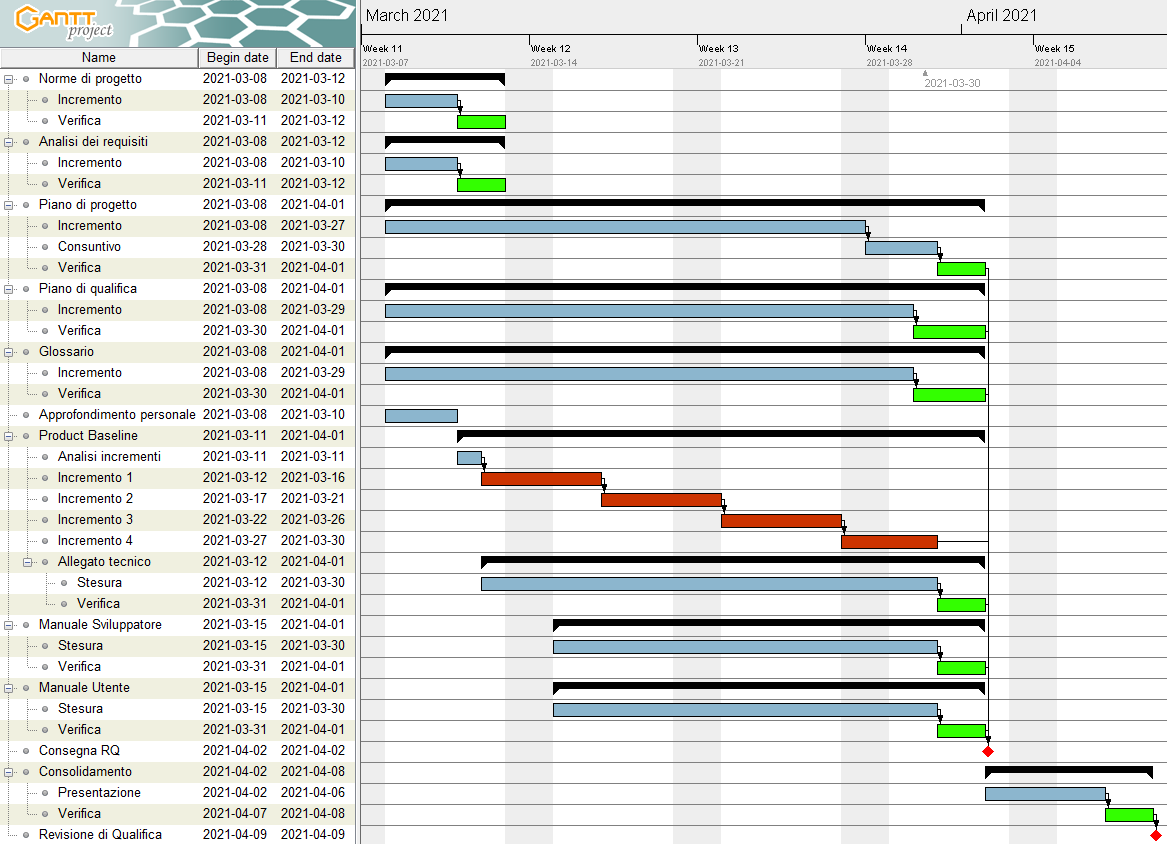
\includegraphics[scale=0.6]{res/Pianificazione/Gantt/codifica}}
\caption{Diagramma di Gantt per il periodo di progettazione di dettaglio e codifica}
\end{figure}

Per migliorare la visualizzazione del diagramma, la pianificazione dei singoli incrementi viene rappresentata dal successivo diagramma, che ha una durata di 5 giorni. L'ultimo incremento è pianificato per solo 4 giorni poiché prevediamo non sia così impegnativo rispetto agli altri, che richiedono molta più codifica.\\

\begin{figure}[H]
\centering

\centerline{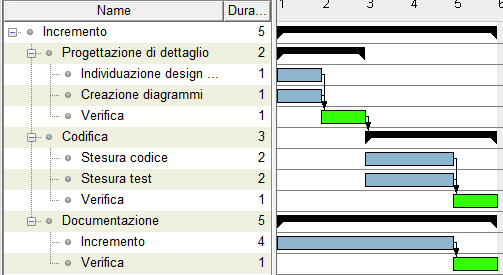
\includegraphics[scale=1]{res/Pianificazione/Gantt/incCodifica.PNG}}
\caption{Diagramma di Gantt per i singoli incrementi nel periodo di progettazione di dettaglio e codifica}
\end{figure}
